
\documentclass[12pt]{article}

% Layout.
\usepackage[top=1in, bottom=0.75in, left=1in, right=1in, headheight=1in, headsep=6pt]{geometry}

% Fonts.
\usepackage{mathptmx}
\usepackage[scaled=0.86]{helvet}
\renewcommand{\emph}[1]{\textsf{\textbf{#1}}}

% TiKZ.
\usepackage{tikz, pgfplots}
\usetikzlibrary{calc}
\pgfplotsset{compat = newest}
 
\pgfplotsset{my style/.append style={axis x line=middle, axis y line=
middle, xlabel={$x$}, ylabel={$y$}, axis equal }}

% Misc packages.
\usepackage{amsmath,amssymb,latexsym}
\usepackage{graphicx}
\usepackage{array}
\usepackage{xcolor}
\usepackage{multicol}

% Commands to set various header/footer components.
\makeatletter
\def\doctitle#1{\gdef\@doctitle{#1}}
\doctitle{Use {\tt\textbackslash doctitle\{MY LABEL\}}.}
\def\docdate#1{\gdef\@docdate{#1}}
\docdate{Use {\tt\textbackslash docdate\{MY DATE\}}.}
\def\doccourse#1{\gdef\@doccourse{#1}}
\let\@doccourse\@empty
\def\docscoring#1{\gdef\@docscoring{#1}}
\let\@docscoring\@empty
\def\docversion#1{\gdef\@docversion{#1}}
\let\@docversion\@empty
\makeatother

% Headers and footers layout.
\makeatletter
\usepackage{fancyhdr}
\pagestyle{fancy}
\fancyhf{} % Clears all headers/footers.
\lhead{\baselineskip 30pt
%\emph{\@doctitle\hfill\@docdate}
\emph{\@docdate\hfill\@doctitle}
\ifnum \value{page} > 1\relax\else\\
\emph{Name: \rule{3.5in}{1pt}\hfill \@docscoring}\fi}
\rfoot{\emph{\@docversion}}
\lfoot{\emph{\@doccourse}}
\cfoot{\emph{\thepage}}
\renewcommand{\headrulewidth}{0pt}%
\makeatother

% Paragraph spacing
\parindent 0pt
\parskip 6pt plus 1pt

% A problem is a section-like command. Use \problem{5} to
% start a problem worth 5 points.
\newcounter{probcount}
\newcounter{subprobcount}
\setcounter{probcount}{0}
\newcommand{\problem}[1]{%
\par
\addvspace{4pt}%
\setcounter{subprobcount}{0}%
\stepcounter{probcount}%
\makebox[0pt][r]{\emph{\arabic{probcount}.}\hskip1ex}\emph{[#1 points]}\hskip1ex}
\newcommand{\thesubproblem}{\emph{\alph{subprobcount}.}}

% Subproblems are an enumerate-like environment with a consistent
% numbering scheme. 
% Use \begin{subproblems}\item...\item...\end{subproblems}
\newenvironment{subproblems}{%
\begin{enumerate}%
\setcounter{enumi}{\value{subprobcount}}%
\renewcommand{\theenumi}{\emph{\alph{enumi}}}}%
{\setcounter{subprobcount}{\value{enumi}}\end{enumerate}}

% Blanks for answers in normal and math mode.
\newcommand{\blank}[1]{\rule{#1}{0.75pt}}
\newcommand{\mblank}[1]{\underline{\hspace{#1}}}
\def\emptybox(#1,#2){\framebox{\parbox[c][#2]{#1}{\rule{0pt}{0pt}}}}

% Misc.
\renewcommand{\d}{\displaystyle}
\newcommand{\ds}{\displaystyle}
\def\bc{\begin{center}}
\def\ec{\end{center}}
\def\be{\begin{enumerate}}
\def\ee{\end{enumerate}}


\doctitle{Math 251: Quiz 8}
\docdate{March 27, 2025}
\doccourse{UAF Calculus I}
\docversion{v-1}
\docscoring{\blank{0.8in} / 25}
\begin{document}

There are 25 points possible on this quiz. No aids (book, calculator, etc.)
are permitted.  {\emph{Show all work for full credit.}}

\problem{11} Let $\ds g(x) = \frac{3}{2}x^4-3x^3$. Note that we have
the following:
$$
g'(x) = 6x^3 - 9x^2 \hspace{3cm} g''(x) = 18x^2-18x
$$

{\bf You must show your work for all parts to receive credit!}
\begin{subproblems}
\item Determine the intervals where $g$ is {\bf increasing} and where
  $g$ is {\bf decreasing}.
  \vfill

\item Find the $x$ values where any {\bf local maxima} occur and where any
  {\bf local minima} occur.
  \vfill

\item Find the intervals where $g$ is {\bf concave up} and where $g$ is
  {\bf concave down}.
  \vfill

\item Find the $x$ values where any {\bf inflection points} occur.
  \vfill
\end{subproblems}

\newpage

\problem{8} Evaluate the following limits. {\bf Show your work!}
\begin{subproblems}
\item $\ds \lim_{x \rightarrow -\infty} \frac{x^2+1}{x^2-2x^3}$
  \vfill

\item $\ds \lim_{x \rightarrow \infty} \frac{4x-2}{\sqrt{5x^2-4}}$
  \vfill
\end{subproblems}

\problem{6} Based on the graph of the function $f(x)$ below, determine
whether each value is positive, negative, zero, or undefined. You do
not need to show your work.
\begin{multicols}{2}
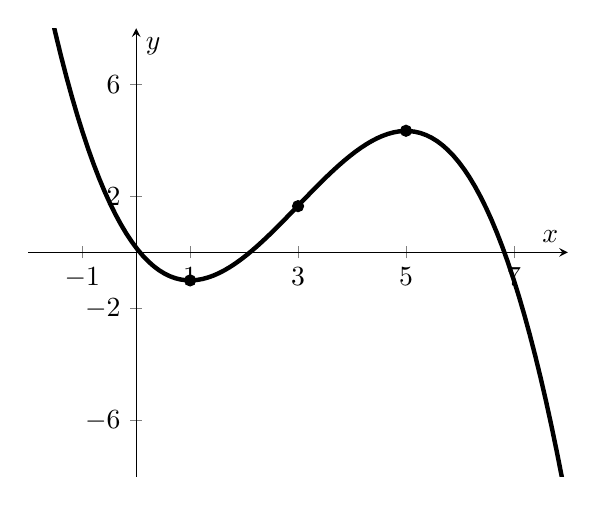
\begin{tikzpicture}
 \begin{axis}[
    xmin = -2, xmax = 8,
    ymin = -8, ymax = 8, xtick={-3,-1,...,7}, ytick={-6, -2,...,6},axis x line=middle, axis y line=
middle, xlabel={$x$}, ylabel={$y$}]
    \addplot[ultra thick, <->,samples=100,
        domain = -2:8,
    ] {-1+(x-1)*(x-1)-(1/6)*(x-1)*(x-1)*(x-1)};
    \addplot[mark=*,only marks] coordinates {(1,-1)(3,1.65)(5,4.34)};
\end{axis}
\end{tikzpicture}

\columnbreak

\begin{subproblems}
\item $g'(1)$
\item $g''(1)$
\item $g'(3)$
\item $g''(3)$
\item $g'(5)$
\item $g''(5)$
\end{subproblems}
\end{multicols}


\end{document}
%%% Local Variables:
%%% mode: LaTeX
%%% TeX-master: t
%%% End:
